\documentclass[en]{../../../../../../eplexam}

\usepackage{../../../../../../eplunits}

\hypertitle{Optics and lasers}{7}{PHYS}{2143}{2020}{Janvier}{All}
{Martin Braquet}
{Alain Cornet, Baptiste Fabre et Clément Lauzin}

A manually written recto-verso formulary is authorized (4h exam).

\section{Theory}

Give an answer to four of the six following questions:

\begin{enumerate}
 \item Explain why the propagation of light is directed towards the increasing refraction indexes.
 \item Explain the experiment of Bessel to compute the focal length of a lens. Provide the demonstration and the limitations of this experiments.
 \item Describe one transfer function in Fourier optics.
 \item Explain the use of a compensating plate for a Michelson interferometer.
 \item In a Fabry-Perot cavity, describe the finesse and its equation.
 \item 
\end{enumerate}

\nosolution

\section{Exercice: Young's holes}

Description of the Young's holes experiment: a source $S$ is split in two sources $S_1$ and $S_2$. The axes are as follows: $x$ is the axis of the two sources, $z$ is the longitudinal axis (from the source to the point) and $y$ is the second axis on the source plane (perpendicular to the axis of $S_1$ and $S_2$).

\begin{enumerate}
 \item Give the expression of the path difference between the two sources towards a point $M$ on the screen.
 \item Deduce the order of interference and the intensity distribution.
 \item Give the position of the central peak of intensity.
\end{enumerate}

We now move the source $S$ on the $y$ axis.

\begin{enumerate}
 \item Is there a difference in the path difference.
 \item Prove with this results that it is possible to use slits instead of holes. What is the advantage?
\end{enumerate}

We now replace the source $S$ at $y=0$, and place a small medium of refractive index $n$ in front of the first source $S_1$. Its width is $e$ and we suppose that the light travels this distance $e$ in the medium since the angles are small (the point $M$ is far).

\begin{enumerate}
 \item Give the expression of the new path difference and deduce the order of interference.
 \item Give the position of the central peak of intensity.
\end{enumerate}

We place another piece of medium $n'$ and width $e'$ in front of the second source $S_2$.

\begin{enumerate}
 \item Give the expression of the new path difference.
 \item Find the value of the width $e'$ such that the central peak is brought back at the origin. Numerical application: $n=1.5$, $n'=1.7$ and $e=\SI{420}{\micro m}$.
\end{enumerate}

\nosolution

\section{Laser cavity}

We consider a gamma laser cavity with two plane mirrors $M_2$ and $M_4$, and two convex mirrors $M_1$ and $M_3$ with the same radius of curvature $R$.

\begin{figure}[H]
 \centering
 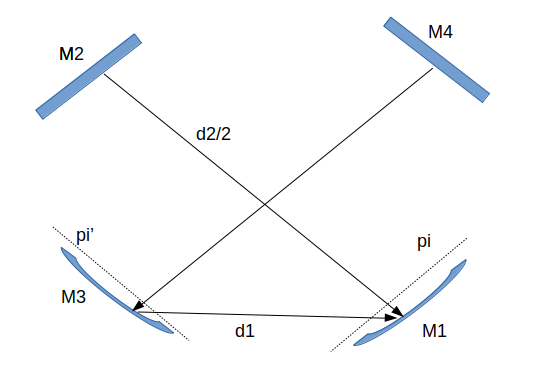
\includegraphics[width=0.7\textwidth]{img/laser.png}
\end{figure}

\begin{enumerate}
 \item Give the transfer matrix $T_{\pi \rightarrow \pi'}$ starting from $\pi$ towards $M_2$ and ending at $\pi'$ after the reflection on $M_3$.
 \item We consider that $d_1=\SI{30}{cm}$, $d_2/2=\SI{50}{cm}$ and $R=\SI{50}{cm}$. Give the numerical value of the transfer matrix by keeping the fractional values.
 \item Describe the full path of a wave on this cavity and compute the total transfer matrix $T_{\pi \rightarrow \pi}$ in function of $T_{\pi \rightarrow \pi'}$.
 \item Ensure that you obtain 
 \[
  T_{\pi \rightarrow \pi} = \left(\begin{array}{cc}
                             \frac{-39}{25} & \frac{-11}{25}\\
                             \frac{32}{25} & \frac{-7}{25}
                            \end{array}\right)
 \]
 with the numerical values.
 \item BONUS: Find and explain the stability of this cavity.
 \item BONUS: Give and explain the number and the positions of the expected waists in this cavity.
\end{enumerate}


\end{document}
